\documentclass[a4paper]{article}

\usepackage[T1]{fontenc}
\usepackage[italian]{babel}
\usepackage[utf8x]{inputenc}
\usepackage{graphicx}



\begin{document}
	\title{Interferometro di Michelson}
	\maketitle
	
	\begin{abstract}
		 Misura della lunghezza d'onda di tre diversi laser.
		 
		 Misura di spostamenti micrometrici: isteresi di un piezoelettrico.
		 
		 Misura dell'indice di rifrazione dell'aria
	\end{abstract}

\section{Apparato sperimetale}

\section{Teoria}
\begin{center}
	\begin{minipage}[c]{.50\textwidth}
		\centering
		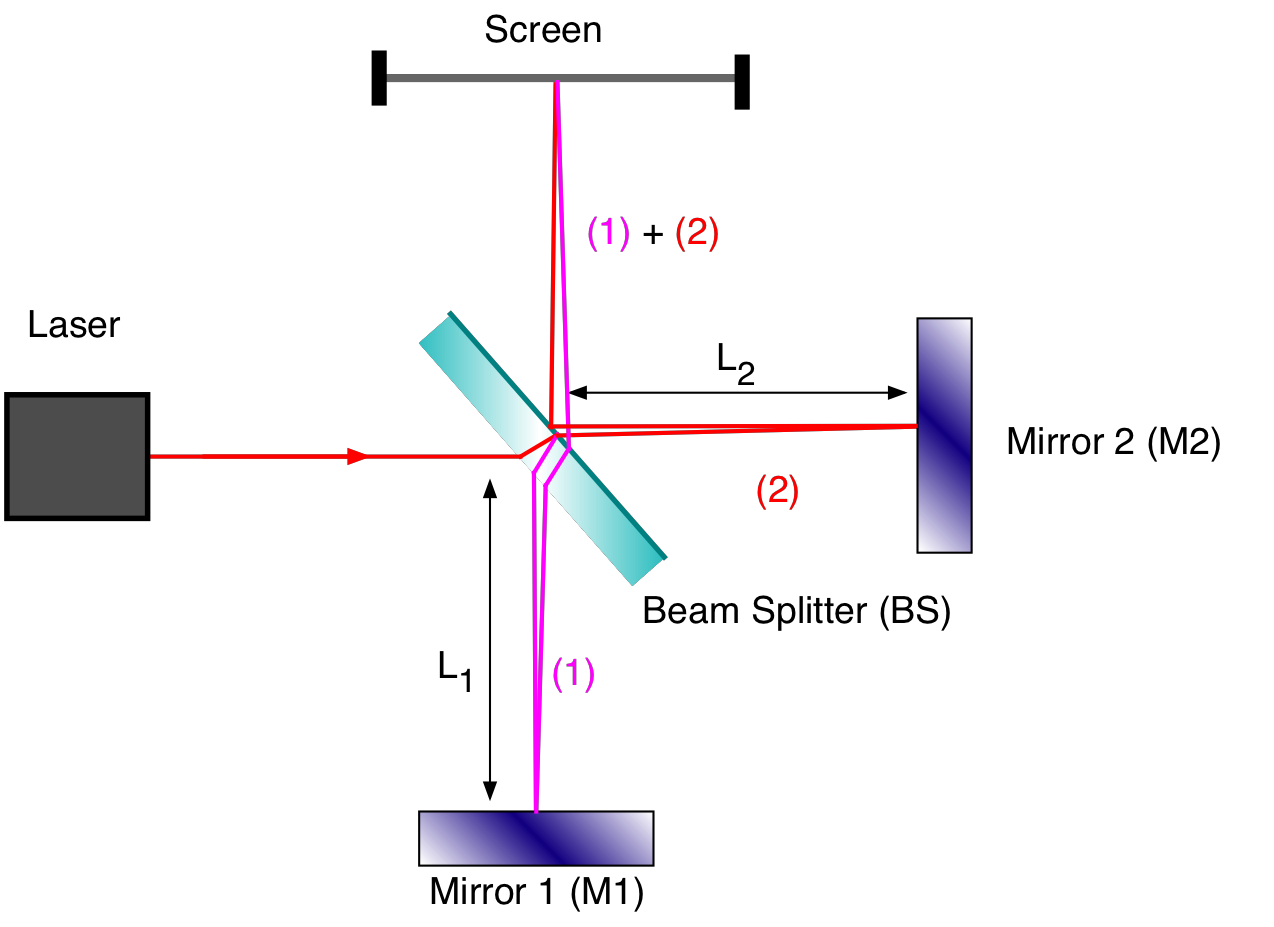
\includegraphics[width=1\textwidth]{michelson.png}
	\end{minipage}
	\begin{minipage}[c]{.40\textwidth}
		In un interferometro di Michelson come quello in figura la condizione per avere interferenza costruttiva è $2(L_1 -L_2) = m \lambda$. Nel nostro apparato contiamo il numero $m$ di frange al variare di $L_2$. 
	\end{minipage}
\end{center}
	

\section{Misura della lunghezza d'onda}

\section{Isteresi del piezoelettrico}

\section{Indice di rifrazione dell'aria}


\end{document}
